\documentclass[a4paper,norsk,12pt]{article}
\usepackage[utf8]{inputenc}

% Oppsett for norsk
\usepackage[norsk]{babel}
\usepackage{times}
\usepackage[T1]{fontenc}
\usepackage{parskip}
\DeclareUnicodeCharacter{00A0}{ }
\newcommand{\strek}{\textthreequartersemdash}

% Andre pakker
\usepackage{oving}
\usepackage{amsmath}
\usepackage{amssymb}
\usepackage{varioref}
\usepackage{subcaption}
\usepackage{units}
\usepackage{todo}

\def \oppgavename {Problem}

% Roman numerals
\makeatletter
\newcommand*{\rom}[1]{\expandafter\@slowromancap\romannumeral #1@}
\makeatother


\title{MAT200 --- Mathematical Methods 2}
\subtitle{Compulsory Assignment 1}
\author{Christian Stigen}
\date{UiS, 19.~februar, 2016}

\begin{document}
\maketitle
\oppgave{1 (i)}
The radicand must be zero or greater, or
\begin{align*}
  0 & \leqslant x^2-6x+\frac{1}{4}y^2 \> \Big{|} \cdot-4, +y^2 \\
  y^2 & \geqslant 4x(6-x)
\end{align*}
The right-hand side is zero for $x=0$ and $x=6$, and negative for $x<0$
and $x>6$. Thus, the inequality is true for $0 < x < 6$.

For plotting $\mathcal{D}(f)$, we note that
  \begin{align}
    y_{-} \leqslant -2\sqrt{x(6-x)} & \wedge y_{+} \geqslant 2\sqrt{x(6-x)}
    \,\text{for}\, 0<x<6 \label{eq.1i}
  \end{align}
In fact, taken together, they form an ellipse---see figure \vref{plot.p1}.

\oppgave{1 (ii)}

$C=0$ is given by (\ref{eq.1i}) above,
\begin{align*}
  f(x,y) = \sqrt{x^2 - 6x + \frac{1}{4}y^2} &= 0\\
  x^2 - 6x + \frac{1}{4}y^2 &= 0\\
  y = \pm2\sqrt{x(6-x)} \, \text{for} \, &0 \leqslant x \leqslant 6
\end{align*}
$C=4$ is given by
\begin{align*}
  f(x,y) &= \sqrt{x^2 - 6x + \frac{1}{4}y^2} = 4\\
  \frac{1}{4}y^2 &= 16 - x^2 + 6x\\
  y &= \pm2\sqrt{(x+2)(8-x)}
\end{align*}

The plot of these two level-curves (or \textit{contour curves}) is given in
figure \vref{plot.p2}. Note that we could have used scaling and shifting, which
is much easier, but I felt like doing it this way for fun.

\oppgave{1 (iii)}
Any level-curve is defined by $f(x,y)=C$. For the one corresponding to $(5,6)$,
we could insert $x_0=5$ and $y_0=6$ and find $C$, but we don't need to: When we
perform implicit differentiation of the resulting expression---to find the
slope in $(5,6)$, or any point, in fact---we see that $C'=0$. Therefore we go
straight to differentiation.
\begin{align*}
  C &= x^2 - 6x + \frac{1}{4}y^2 \\
  0 &= 2x - 6 + \frac{1}{2}yy' \\
  y' &= \frac{12-4x}{y} \\
  y'(5,6) &= -\frac{4}{3}
\end{align*}
Now that we have the slope, we can find the tangent line going through this
point by back-calculating the $y$-value for $x=0$ to find $\ell$.
\begin{align*}
  \ell_{(x_0, y_0)} &= y_0 - x_0y'(x_0,y_0) + y'(x_0,y_0)x \\
  \ell_{(5,6)} &= 6+\frac{4\cdot5}{3} -\frac{4}{3}x \\
  \ell_{(5,6)} &= -\frac{4}{3}x +\frac{38}{3}
\end{align*}
This is plotted in figure \vref{plot.p3}.

\oppgave{2 (i)}
\begin{align*}
  f(x,y,z) &= e^z + e^{2y}\arctan{\left(\frac{y}{x}\right)} \\
  \\
  % df/dx
  \frac{\partial f}{\partial x} &=
    e^{2y}\frac{1}{\frac{x^2}{y^2}+1} \left(\frac{-y}{x^2}\right)
      = \frac{-ye^{2y}}{x^2+y^2} \\
  \\
  % df/dy
    \frac{\partial f}{\partial y} &= \frac{\partial}{\partial y}(uv) =
    u'v+uv' \,\text{where}\, u=e^{2y} \,\text{and}\, v=\arctan{\frac{y}{x}}
    \\
    &= 2e^{2y}\arctan{\left(\frac{y}{x}\right)} + \frac{e^{2y}}{1+\frac{y^2}{x^2}}\cdot\frac{1}{x}
    = 2e^{2y}\arctan{\left(\frac{y}{x}\right)} + \frac{xe^{2y}}{x^2+y^2} \\
    \frac{\partial f}{\partial z} &= e^z
\end{align*}

\oppgave{2 (ii)}
\begin{align*}
  % d^2f/dx^2
  \frac{\partial^2 f}{\partial x^2} &=
  \frac{\partial}{\partial x} \left(\frac{-ye^{2y}}{x^2+y^2}\right)
    = \frac{2xye^{2y}}{(x^2+y^2)^2}
  \\
  \\
  % d^2f/(dx dy)
  \frac{\partial^2 f}{\partial x \partial y} &=
  \frac{\partial}{\partial x} \left(\frac{\partial f}{\partial y}\right) =
    \frac{\partial}{\partial x} \left( 
      2e^{2y}\arctan{\left(\frac{y}{x}\right)} + \frac{xe^{2y}}{x^2+y^2}
    \right)
    \\
    &= \frac{-2ye^{2y}}{x^2+y^2} + \frac{e^{2y}(x^2+y^2)-xe^{2y}\cdot2x}{(x^2+y^2)^2}
    = -e^{2y}\frac{2y(x^2+y^2) - (x^2+y^2) + 2x^2)}{(x^2+y^2)^2} \\
    &= -\frac{e^{2y}}{(x^2+y^2)^2}\left( 2yx^2 + 2y^3 -x^2 - y^2 + 2x^2 \right)
    \\
    &= -\frac{e^{2y}}{(x^2+y^2)^2}\left( y^2(2y-1) + x^2(2y+1) \right)
\end{align*}

\oppgave{2 (iii)}
\begin{align*}
  g(s,t) &= f(s, st, s+t) = e^{s+t} + e^{2st}\arctan{t} \\
  \\
  \frac{\partial g}{\partial s} &= e^{s+t} + 2te^{2st}\arctan{t} \\
  \\
  \frac{\partial g}{\partial t} &= e^{s+t} + (uv)' \,\text{where}\, u=e^{2st}
    \,\text{and}\, v=\arctan{t} \\
    &= e^{s+t} + u'v + u+v' \\
    &= e^{s+t} + 2se^{2st}\arctan{t} + \frac{e^{2st}}{1+t^2}
\end{align*}

\oppgave{3 (i)}
To find the tangent plane, we must find $F_x = \frac{\partial F}{\partial x}$
and $F_y = \frac{\partial F}{\partial y}$. We start by organizing $F$, setting
$g=xy-\frac{\pi}{4}$ and getting $g'_x=y$ and $g'_y=x$.
%
\begin{align*}
  F &= (2y-2x)\sin^2{(xy-\frac{\pi}{4})}
      = 2y\sin^2{(xy-\frac{\pi}{4})} - 2x\sin^2{(xy-\frac{\pi}{4})} \\
      &= 2y\sin^2{g}-2x\sin^2{g} \\
\\
  F_x &= 0+2y^22\sin{g}\cos{g} -2\sin^2{g} - 2xy2\sin{g}\cos{g} \\
      &= 2y^2\sin{2g} - 2\sin^2{g} - 2xy\sin{2g} \\
      &= 2y(y-x)\sin{2g} - 2\sin^2{g} \\
\\
  F_y &= 2\sin^2{g} + 2y2x\sin{g}\cos{g} - 0 - 2x2x\sin{g}\cos{g} \\
      &= 2\sin^2{g} + x\sin{2g}(2y-2x)
\end{align*}
Inserting the point $(0,2)$ gives
\begin{align*}
  g(0,2) &= -\frac{\pi}{4} \\
  F_x(0,2) &= 8\sin{-\frac{\pi}{2}} - 2\sin^2{-\frac{\pi}{4}} = -8-1 = -9 \\
  F_y(0,2) &= 1 \\
  F(0,2) &= 2(2-0)\sin^2{(0-\frac{\pi}{4})} = 4\sin^2{(-\frac{\pi}{4})} = 2
\end{align*}
The tangent plane $T$ is given by
\begin{align*}
  T - F(a,b) &= F_x(a,b)(x-a) + F_y(a,b)(y-b) \\
  T + 2 &= xF_x(0,2) + F_y(0,2)(y-2)
\end{align*}
Plugging in the above values, we get the tangent plane equation.
\begin{align*}
  T - 2 &= xF_x(0,2) + F_y(0,2)(y-2) \\
        &= -9x + y - 2 \\
  T &= y-9x
\end{align*}

\oppgave{3 (ii)}
Using the tangent equations as the component slopes of $F$ at a point $(x_0,
y_0)$, the linear approximation is given by
\begin{align*}
  L(x,y) &= F(x_0, y_0) + F_x(x_0, y_0)(x-x_0) + F_y(x_0, y_0)(y-y_0)
\end{align*}
We'll choose the point $(x_0, y_0) = (-1, 0)$ to approximate $F(-1.05, 0.02)$.
\begin{align*}
  F(x,y) \approx
  L_{(-1,0)}(x,y)
    &= F(-1,0) + F_x(-1,0)(x+1) + F_y(-1,0)(y) \\
    &= 1 - x - 1 + 3y = 3y-x \\
  L_{(-1,0)}(-1.05, 0.02)
    &= 3\cdot0.02 + 1.05 = 1.11
\end{align*}
For comparison, the correct value $F(-1.05, 0.02) \approx 1.11493$, so the
approximation seems reasonable. Of course, we could have used the tangent plane
equation from the previous problem directly. At $(-1,0)$, it is
\begin{align*}
  T_{(-1,0)}(x,y)
    &= F_x(-1,0)(x+1) + F_y(-1,0)(y-0) + F(-1,0)\\
    &= -x-1 + 3y + 1 = 3y-x
\end{align*}
The two methods are exactly the same.

\clearpage
\oppgave{3 (iii)}
We could simply use $f'(x) = -\frac{F_x}{F_y}$, as we have done in 3 (iv), but
I wanted to do it the other, hard way as well.

First we need some helper equations:
\begin{align*}
  u &= xy-\frac{\pi}{4} \\
  \sin^2{u} &= \frac{1-\cos{2u}}{2}
      \iff \cos{2u} = 1 - 2\sin^2{u} \\
  2\sin{u}\cos{u} &= \sin{2u} \\
  u' &= xy' + y \\
  \sin^2{u}' &= 2\sin{u}\cos{u}\cdot u' = \sin{2u}(xy'+y) =
      xy'\sin{2u}+y\sin{2u}
\end{align*}
Simplifying $F(x,y)-1 = 0$,
\begin{align*}
  2(y-x)\left(\frac{1-\cos{2u}}{2}\right) &= 1 \\
  (y-x)(1-\cos{2u}) &= 1
\end{align*}
Multiplying out
\begin{align*}
  (y-x)(1-\cos{2u}) &= 1 \\
  y - y\cos{2u} -x + x\cos{2u} &= 1
\end{align*}
Differentiating both sides using above helpers,
\begin{align*}
  y' - y'\cos{2u} + y\sin{2u}\cdot 2u' - 1 + \cos{2u} - x\sin{2u}\cdot 2u' &= 0 \\
  y' - y'\cos{2u} + 2y\sin{(2u)}(y+xy') - 1 + \cos{2u} - 2x\sin{(2u)}(y+xy') &= 0 \\
  y' - y'\cos{2u} + 2y^2\sin^2{u} + 2xyy'\sin{2u} - 1 + \cos{2u}
    +2xy\sin{2u} + 2x^2y'\sin{2u} &= 0
\end{align*}
Grouping $y'$-terms on the left, rest on the right,
\begin{align*}
  y'\left( 1 - \cos{2u} + 2xy\sin{2u} - 2x^2\sin{2u} \right)
    &= -2y^2\sin{2u} + 2xy\sin{2u} + 1 - \cos{2u} \\
\end{align*}
Dividing and reorganizing using $\cos{2u} = 1 - 2\sin^2{u}$,
\begin{align*}
  y' &= \frac{-2y^2\sin{2u} + 2xy\sin{2u} + 1 - \cos{2u}}
             {1 - \cos{2u} + 2xy\sin{2u} - 2x^2\sin{2u}}
      = \frac{-2y(y-x)\sin{2u} + 1 - 1 + 2\sin^2{u}}
             {1 - 1 + 2\sin^2{u} + x\sin{2u}(2y-2x)}
\end{align*}
Finally, we get the \textit{exact} same result as in 3 (iv).
\begin{align*}
  y' &= \frac{-2y(y-x)\sin{2u} + 2\sin^2{u}}
             {2\sin^2{u} + x\sin{2u}(2y-2x)}
      = \frac{-y(y-x)\sin{2u} + \sin^2{u}}
             {x(y-x)\sin{2u} + \sin^2{u}}
\end{align*}


\oppgave{3 (iv)}
\begin{align*}
  F(0,y) &= 1 \\
  2y\sin^2{-\frac{\pi}{4}} &= 1\\
  y &= 1 \,\text{when}\, F(0,y)=1\\
\end{align*}
We thus have $x=0$ and $y=1$. This gives $2u = -\frac{\pi}{2}$, $\sin{2u} =
-1$, $\cos{2u} = 0$. To find $f'(x)$,
\begin{align*}
  f'(x) &= -\frac{\partial F / \partial x}{\partial F / \partial y}
  = -\frac{F_x}{F_y}
\end{align*}
This is true because $F_x$ and $F_y$ are not altered by adding a constant $-1$,
because $\frac{\partial}{\partial x}\left(-1\right) = 0$ and the same for
$\frac{\partial}{\partial y}$. Therefore we get
\begin{align*}
  f'(x) &= \frac{
      -2y(y-x)\sin{(2g)}+2\sin^2{(g)}
    } {
      2\sin^2{(g)}+x\sin{(2g)}(2y-2x))
    }
\end{align*}
Inserting $x=0$, we get
\begin{align*}
  f'(0) &= \frac{-2y^2\cdot-1 + 2\cdot\frac{1}{2}}{2\cdot\frac{1}{2}+0}
\end{align*}
But we already found that $y(0)=1$ for $F(0,y)=1$, so we insert $y=1$ in the
above and get
\begin{align*}
  f'(0) &= \frac{2\cdot1 + 1}{1} = 3
\end{align*}

\begin{figure}[h]
  \centering
  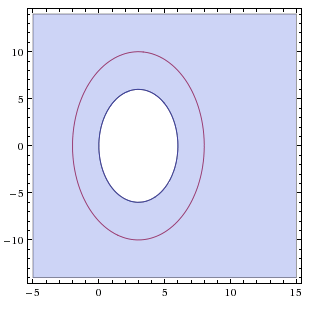
\includegraphics{ob1plot2.png}
  \caption{Problem 1 (i) and (ii): Light blue area is $\mathcal{D}(f)$,
           dark blue line is $C=0$ and purple line is $C=4$.}
  \label{plot.p2}
  \label{plot.p1}
\end{figure}

\begin{figure}[h]
  \centering
  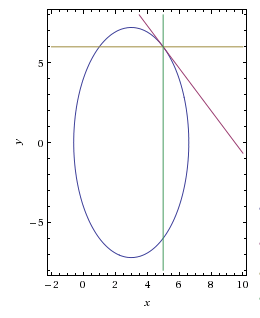
\includegraphics{ob1plot3.png}
  \caption{Plot of tangent line $\ell_{(5,6)}$ in problem 1 (iii).}
  \label{plot.p3}
\end{figure}

\end{document}
